\section{What context must do, and the evidence}
\label{sec:row-0}

We meet the running example, define the input to one model call, what it must do and what it costs, map the research on long context, and look at one experiment on how models use long inputs.

\subsection{Part II follows one agent's vending business}
\label{sec:it-5-0}

\bi
\item \textbf{The business:} an agent orders stock for a vending machine and sets prices.
\item \textbf{The order:} on Day 1 it pays for 10 units of SKU-A, due on Day 4.
\item \textbf{The history:} each day adds tool results and log lines until the window is full.
\item \textbf{The question:} on Day 4, the next call must still see the order paid on Day 1.
\ei

This is the running example of Part II. Its records, its days and its question repeat in most of the figures that follow, up to the dropped order of the long-horizon section and the evaluation. The task comes from Vending-Bench (Axel Backlund and Lukas Petersson, Andon Labs, arXiv:2502.15840, 2025, a preprint), which the long-horizon section presents: an agent runs a vending-machine business over simulated days. It checks inventory, orders stock, sets prices and pays a daily fee, and an order arrives some days after the agent places it.

The records are the course's. A SKU, short for stock-keeping unit, is the code a retailer gives one product, so SKU-A is one product in the machine. The inventory-ledger holds the agent's orders and payments, and the ops-log holds what happened at the machine each day. On Day 1 the agent pays 30.00 for 10 units of SKU-A, due on Day 4. On Days 2 and 3 the shelf stays empty and nothing sells.

Every day adds tool calls, tool results and log lines to the history, and the model sees the history only through its window. In the teaching case the window is full by Day 3, so the harness must compact or select before Day 4. On Day 4 the agent decides whether to order SKU-A again. The only record that says more SKU-A is on the way is the Day 1 ledger line, so a context without it leads the agent to order again and pay twice. Part II asks what each call must see so that the run keeps commitments like this one, and how to compact the history without losing them.

The whole run, its records, the price, the days and the window meter are the course's illustrative teaching case, and the meter counts no tokens. Vending-Bench supplies the task and its daily fee, and the course supplies the ledger and log lines that the later figures quote.

\begin{figure}[htbp]
\centering
\includegraphics[width=\linewidth]{context/vending-run-4.png}
\caption{Part II follows one agent's vending business. The figure as it stands after the build's last click.}
\label{fig:vending-run-4}
\end{figure}

\paragraph{The figure, stage by stage.}
\be
\item The business: the agent's tool calls reach the vending machine and its suppliers, and it ``checks inventory, orders stock, sets prices, pays a daily fee''. The three dashed bands wait for Day 1, Days 2 and 3, and Day 4, and the grey note marks the run as the course's teaching case.
\item Day 1: the agent orders and pays, and the inventory-ledger records ``Day 1: ordered 10 SKU-A'' and ``paid 30.00, due Day 4''. The navy caption says what the code means: ``SKU-A: a stock-keeping unit, the code of one product''.
\item Days 2 and 3: the ops-log records ``Day 2: shelf empty, no sales'' and ``Day 3: shelf empty, no sales'', and the meter shows the history of Days 1, 2 and 3 filling the window: ``the history fills the window''.
\item Day 4: ``the next call must answer 'is more SKU-A already on the way?'''. The Day 1 ledger line turns navy, because ``the answer is the Day 1 ledger line, so the call must still see it''.
\ee

\begin{takeaway}Part II asks what each call must see so that the run keeps its commitments.\end{takeaway}

\subsection{Context supplies each call within a budget}
\label{sec:it-5-1}

\bi
\item \textbf{Input:} instructions, history and selected records enter one model call.
\item \textbf{Objective:} the next decision needs correct facts, intact meaning and a route to the source.
\item \textbf{Cost:} each call fits a window, and every call sends its context again.
\ei

The records in the figure are those of the running example on the previous slide.

Every call to the model receives one input, its context: the instructions and tool definitions, the history of messages and tool results, and any source material the harness selects. Every other record stays outside the call. The next decision needs correct facts, their meaning intact, and a route back to the source. Each call fits a window, and the run pays for the context again on every call, so the budget belongs to the run as well as to the call. Repeated history, summaries and retrievals all add tokens, time and charges across the run.

Prithvi Rajasekaran, Ethan Dixon, Carly Ryan and Jeremy Hadfield, of Anthropic's Applied AI team, describe context engineering as the selection of the tokens that go into inference (Effective context engineering for AI agents, Anthropic, September 29, 2025). That article is engineering guidance. Pan et al., LLMLingua-2 (Findings of ACL 2024, section 3.1), discusses token reduction, information content and faithfulness. Source access as a design objective is the course's addition.

Token counts alone do not set the charges: vendors can price cached input and other operations differently, so we define a course budget before we compare alternatives. The evaluation section returns to these objectives, and the long-horizon section uses the difference between a call's capacity and the run's cost.

The records, the 128k window, the 80k input and the five calls in the figure are illustrative. The ledger and log lines are the course's teaching case in the Vending-Bench task, and the figure draws tokens only, so the time and the charges rest on what we say.

\begin{figure}[htbp]
\centering
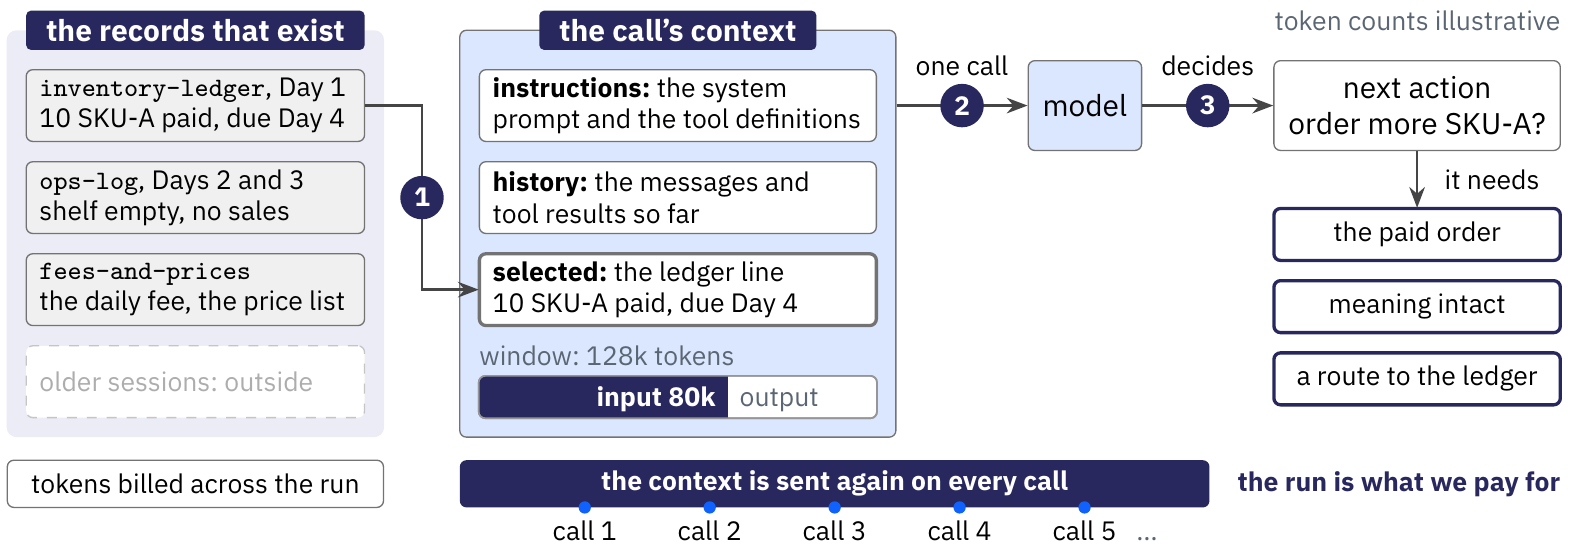
\includegraphics[width=\linewidth]{context/one-call-3.png}
\caption{Context supplies each call within a budget. The figure as it stands after the build's last click.}
\label{fig:one-call-3}
\end{figure}

\paragraph{The figure, stage by stage.}
\be
\item The call's context: arrow 1 selects the ledger line ``10 SKU-A paid, due Day 4'' from ``the records that exist'' and sets it beside the instructions and the history. The window meter shows ``input 80k'' of ``window: 128k tokens'', and the rest of the window is left for the ``output''.
\item The model: arrow 2, ``one call'', sends the context to the model, and arrow 3 shows what it ``decides'', the ``next action'', ``order more SKU-A?''. Under ``it needs'' stand the three things that decision requires from the context: ``the paid order'', ``meaning intact'' and ``a route to the ledger''.
\item The run meter: ``the context is sent again on every call'', from ``call 1'' to ``call 5'' and on, so the ``tokens billed across the run'' add up call after call. The verdict reads ``the run is what we pay for''.
\ee

\begin{takeaway}Context management fits what the next decision needs into the run's budget.\end{takeaway}

\subsection{Long-context research, from models to agents}
\label{sec:it-6-0}

\bi
\item \textbf{Models:} attention, positions and caches make windows longer and cheaper.
\item \textbf{Evaluations:} a model can use less of its window than its makers claim.
\item \textbf{Harnesses:} each call receives a context chosen for its decision.
\item \textbf{Agents:} long runs can produce more history than a window holds.
\ei

The budget of the previous slide has two answers in the research: make the window longer and cheaper, or choose what goes into it. The map places the work Part II builds on. Each lane collects the work that answers one question, and each runs left to right by first public release, the arXiv identifier or the date a test or post appeared. A work keeps the year it first appeared, so Lost in the Middle, which TACL published in 2024, sits at 2023. The reading list at the end of Part II gives every work with its venue and full reference.

The models lane asks how a model can attend to more tokens at lower cost. Transformer-XL (Dai et al., ACL 2019) carries hidden states across segments. Rotary position embedding (Su et al., arXiv 2021, Neurocomputing 2024) is the position scheme of most open models, and YaRN (Peng et al., ICLR 2024) stretches it to longer windows. FlashAttention (Dao et al., NeurIPS 2022) computes exact attention with memory linear in the input length. H2O (Zhang et al., NeurIPS 2023) and StreamingLLM (Xiao et al., ICLR 2024) evict entries from the key-value (KV) cache, the keys and values the model keeps for earlier tokens so that each new token need not recompute them, and the Gemini 1.5 report (Gemini Team, 2024) describes windows of a million tokens and more.

The evaluations lane asks how much of the window a model can use. Passkey retrieval (Mohtashami and Jaggi, NeurIPS 2023) and Needle In A Haystack (Kamradt, 2023, a test on GitHub) hide one fact in filler text. Lost in the Middle, the next slide, moves the evidence. RULER (Hsieh et al., COLM 2024) makes the tasks harder and finds that all but one of the 17 models it tested fall below a fixed score before their claimed length. Its two slides are backups at the end of Part II. HELMET (Yen et al., ICLR 2025) finds that needle scores predict application results poorly, and NoLiMa (Modarressi et al., ICML 2025) removes the literal overlap between the question and the needle, and scores fall.

The harnesses lane asks what each call should receive. RAG (Lewis et al., NeurIPS 2020) retrieves passages for each input. LLMLingua (Jiang et al., EMNLP 2023) and LLMLingua-2 (Pan et al., Findings of ACL 2024) keep the informative tokens. MemGPT (Packer et al., preprint, 2023) pages memory in and out of the window. SWE-agent (Yang et al., NeurIPS 2024) collapses old observations, The Complexity Trap (Lindenbauer et al., NeurIPS 2025 workshop) finds that such masking matches LLM summarization at lower cost, and ACON (Kang et al., ICML 2026) learns guidelines for compressing agent histories.

The agents lane asks what happens as runs grow long. SWE-bench (Jimenez et al., ICLR 2024) poses real GitHub issues in codebases far larger than a window. It is the standard testbed for coding agents, and two works of the harnesses lane, SWE-agent and The Complexity Trap, measure on it. A Vending-Bench run (Backlund and Petersson, preprint, 2025) lasts up to 2,000 messages and more than 20M tokens across its calls, while each call sees the last 30,000 tokens of its history. METR (Kwa et al., NeurIPS 2025) finds that the length of the tasks a model completes half the time, timed by human experts, has doubled about every seven months since 2019, and the long-horizon section draws its chart.

Part II takes the model as given and works in the harnesses lane, with evidence from the evaluations and agents lanes.

Every name on the map is a real work, placed at the year of its first public release, and nothing on it is illustrative. The lanes are the course's grouping: a work sits in the lane of the question it answers. SWE-agent chooses what each call receives, so it is a harness. SWE-bench, the coding agents' testbed, and Vending-Bench sit with the agents, and the evaluations lane holds the tests of one long input. The map shows 23 of the 59 works on the reading list and implies no ranking of influence.

\begin{figure}[htbp]
\centering
\includegraphics[width=\linewidth]{context/literature-map-5.png}
\caption{Long-context research, from models to agents The figure as it stands after the build's last click.}
\label{fig:literature-map-5}
\end{figure}

\paragraph{The figure, stage by stage.}
\be
\item Models, the first lane, in solid navy: Transformer-XL in 2019 carried state across segments, RoPE in 2021 set the position encoding that YaRN stretched in 2023, FlashAttention in 2022 made attention cheaper, H2O and StreamingLLM evict cached entries, and Gemini 1.5 reached a million tokens in 2024. The other three lane names wait in grey.
\item Evaluations: passkey retrieval and Needle In A Haystack hide one fact in filler text, Lost in the Middle moves the evidence, RULER makes the tasks harder, HELMET tests application tasks, and NoLiMa removes the literal overlap between the question and the needle. The window a maker claims and the length a model can use come apart. The models lane settles to lilac.
\item Harnesses: RAG retrieves, LLMLingua and LLMLingua-2 extract, MemGPT pages memory, SWE-agent masks old observations, and the Complexity Trap and ACON measure and learn compression for agents. Each chooses what a call receives. The evaluations lane settles.
\item Agents: SWE-bench sets real GitHub issues in codebases far larger than a window, the testbed of the harness studies. A Vending-Bench run lasts up to 2,000 messages and more than 20M tokens across its calls, while each call sees the last 30,000 tokens of its history. METR's time horizon, the length of task, timed by human experts, that a model completes half the time, has doubled about every seven months. The harnesses lane settles.
\item The four works in navy each have a slide of their own in Part II: Lost in the Middle next, LLMLingua-2 in the strategies segment, and METR's time horizons and Vending-Bench in the long-horizon segment. The rest of the agents lane settles. Part II works in the harnesses lane, with evidence from the evaluations and agents lanes.
\ee

\begin{takeaway}Longer windows still leave each call's context to the harness.\end{takeaway}

\subsection{Evidence position changes accuracy}
\label{sec:it-6-1}

\bi
\item \textbf{Lost in the Middle} (Liu et al., 2024) moves the answer among 20 documents.
\item \textbf{The reported pattern:} accuracy is often highest with the answer first or last, and lowest in the middle.
\item \textbf{The scope:} the models and tasks tested. A present system needs its own test.
\ei

Nelson F. Liu, Kevin Lin, John Hewitt, Ashwin Paranjape, Michele Bevilacqua, Fabio Petroni and Percy Liang, Lost in the Middle: How Language Models Use Long Contexts, Transactions of the Association for Computational Linguistics 12, 157--173, 2024 (doi:10.1162/tacl\_a\_00638). This is one of the sources Part II studies in depth, and the navy work in the evaluations lane of the map on the slide \hyperref[sec:it-6-0]{``Long-context research, from models to agents''}. RULER, its companion, is a backup at the end of Part II. SWE-bench met the same effect on real software tasks: models resolved fewer issues as the retrieved context grew, and its authors cite this paper for it (Jimenez et al., ICLR 2024, section 5).

The study varies the position of the relevant information in multi-document question answering and in key-value retrieval. Performance is often strongest when the relevant information sits near the start or the end of the input, and weaker when it sits in the middle. The finding concerns the models, prompts and tasks the study evaluated, so we do not carry its numbers to current models. A present system needs its own measurement. The open-domain question-answering case study also separates retriever recall from reader accuracy: added retrieved material need not give proportional gains in the answers.

The figure draws the shape of the finding and no values. Its question about Day 4 is the course's example, and its 20 documents are one of the paper's multi-document settings, which also ran 10 and 30 documents with questions from NaturalQuestions-Open. The key-value retrieval task is not drawn. Both ends carry the label ``accuracy high'', which does not mean that they score the same. The result holds for the models and prompts the paper tested in 2023, and no number carries over to current models.

\begin{figure}[htbp]
\centering
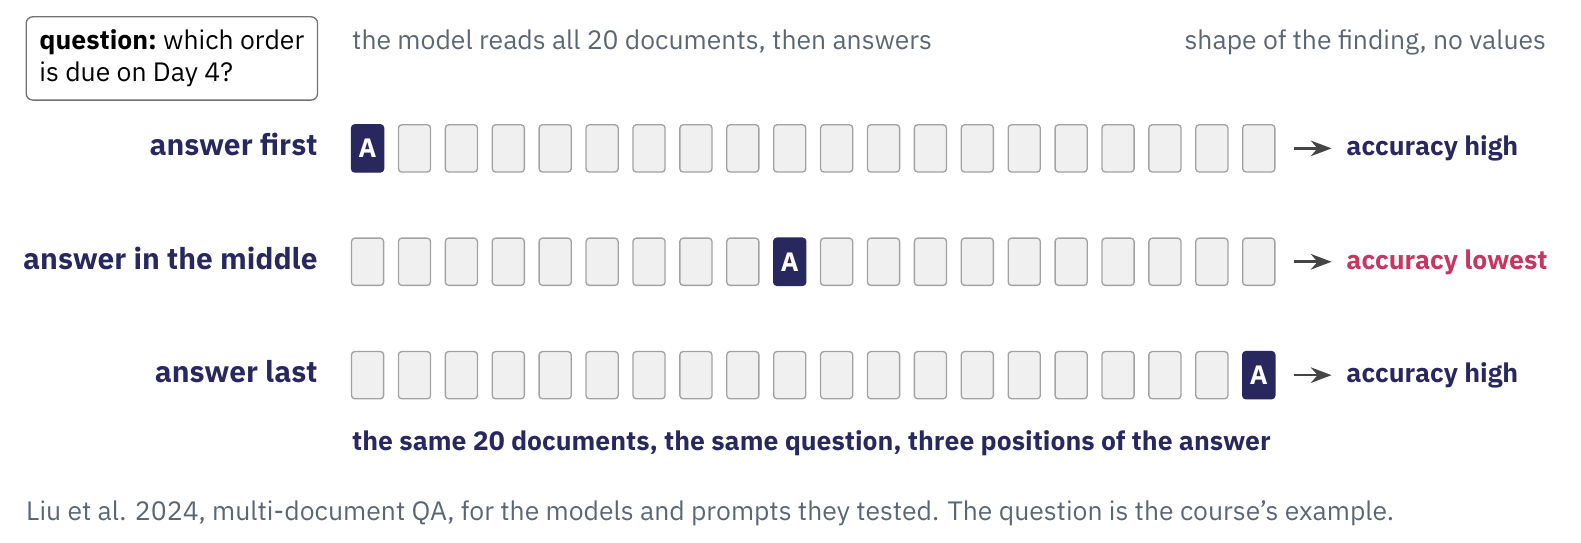
\includegraphics[width=\linewidth]{context/evidence-position-3.png}
\caption{Evidence position changes accuracy. The figure as it stands after the build's last click.}
\label{fig:evidence-position-3}
\end{figure}

\paragraph{The figure, stage by stage.}
\be
\item Answer first: the document marked A holds the answer to 'which order is due on Day 4?' and comes first of the 20. The model reads all 20 documents, then answers, and Liu et al. report accuracy high at this position.
\item Answer in the middle: the same answer document moves to position 10 of the 20. The magenta verdict, accuracy lowest, marks the position where the models and prompts Liu et al. tested answer least accurately.
\item Answer last: the answer document moves to position 20, and the verdict reads accuracy high again. The caption names what stays fixed: the same 20 documents, the same question, three positions of the answer.
\ee

\begin{takeaway}Where evidence sits in the input is a variable each system must test.\end{takeaway}

\subsection*{Key points}
\bi
\item Part II asks what each call must see so that the run keeps its commitments.
\item Context management fits what the next decision needs into the run's budget.
\item Longer windows still leave each call's context to the harness.
\item Where evidence sits in the input is a variable each system must test.
\ei
